\section*{NAIL062 P\&P Logika: Worksheet 3 -- Algebra of propositions, SAT}
% after Lecture 3

\subsection*{Teaching goals:} After completing, the student

\begin{itemize}\setlength{\itemsep}{0pt}
    \item understands the relationship between formulas/theories up to [$T$-]equivalence and sets of models (the so-called algebra of formulas), and can apply this in concrete examples
    \item can encode a given problem as an instance of SAT
    \item has gained practical experience with using a SAT solver
    \item understands the algorithm for solving 2-SAT using the implication graph (including finding all models), and can apply it to an example
    \item understands the algorithm for solving Horn-SAT using unit propagation, and can apply it to an example
    \item understands the DPLL algorithm and can apply it to an example
\end{itemize}


\section*{In-class problems}


\begin{problem}
    
    Let $|\mathbb{P}|=n$ and let $\varphi\in\mathrm{VF}_{\mathbb{P}}$ be a formula such that $|M(\varphi)|=k$. Determine (up to equivalence):
    \begin{enumerate}[(a)]
        \item the number of formulas $\psi$ such that $\varphi \models \psi$ or $\psi \models \varphi$,
        \item the number of theories over $\mathbb{P}$ in which $\varphi$ holds,
        \item the number of complete theories over $\mathbb{P}$ in which $\varphi$ holds,
        \item the number of theories $T$ over $\mathbb{P}$ such that $T \cup \{\varphi\}$ is consistent.
    \end{enumerate}
    Now, consider a contradictory theory $\{\varphi,\psi\}$ where $|M(\psi)|=p$.  Compute (up to equivalence):
    \begin{enumerate}[(a)]\setcounter{enumi}{4}
        \item the number of formulas $\chi$ such that $\varphi \vee \psi \models \chi$, 
        \item the number of theories in which $\varphi \vee \psi$ holds.
    \end{enumerate}

    \begin{solution}
        \begin{enumerate}[(a)]
            \item The condition can be expressed in terms of model sets: $\M(\varphi)\subseteq\M(\psi)$ or $\M(\psi)\subseteq\M(\varphi)$. There are $2^n$ total models, and $|\M(\varphi)|=k$. We want to count possible sets $\M(\psi)$. The condition $\M(\varphi)\subseteq\M(\psi)$ holds for $2^{2^n-k}$ sets (i.e. the number of supersets of the given $k$-element set inside a $2^n$-element universe), and the condition $\M(\psi)\subseteq\M(\varphi)$ holds for $2^k$ sets. We must subtract one to avoid double-counting the case $\M(\psi)=\M(\varphi)$. Altogether there are $2^{2^n-k}+2^k-1$ possible model sets, hence that many formulas $\psi$ up to equivalence.
            \item $T\models\varphi$ iff $\M(T)\subseteq\M(\varphi)$; the number of such model sets $\M(T)$ is $2^k$.
            \item Additionally we require $|\M(T)|=1$; the number of $1$-element subsets of the $k$-element set is $k$.
            \item In terms of models the condition says $\M(T\cup\{\varphi\})\neq\emptyset$. Since $\M(T\cup\{\varphi\})=\M(T)\cap\M(\varphi)$, we count how many possible sets $\M(T)$ have a nonempty intersection with the $k$-element set $\M(\varphi)$. One way to express this is $(2^k-1)\cdot 2^{2^n-k}$, where $2^k-1$ counts the nonempty possible intersections $\M(T)\cap\M(\varphi)$ and $2^{2^n-k}$ counts arbitrary choices for membership of models outside $\M(\varphi)$.
            \item Since $\{\varphi,\psi\}$ is contradictory we have $\emptyset=\M(\varphi,\psi)=\M(\varphi)\cap\M(\psi)$. We count sets $\M(\chi)$ with $\M(\varphi\lor\psi)\subseteq\M(\chi)$. By the Lindenbaum–Tarski algebra $\M(\varphi\lor\psi)=\M(\varphi)\cup\M(\psi)$. Disjointness gives $|\M(\varphi)\cup\M(\psi)|=k+p$, so the number of choices for $\M(\chi)$ is $2^{2^n-(k+p)}$.
            \item $\M(T)$ must be a subset of the $(k+p)$-element set $\M(\varphi\lor\psi)$, hence there are $2^{k+p}$ possibilities.
        \end{enumerate}
                
    \end{solution}
    
\end{problem}


\begin{problem} \label{problem:2sat}
    
    Build the implication graph of the given 2-CNF formula. Is it satisfiable? If yes, find some solution: (a) the formula $\varphi$ below, (b) $\varphi\land\neg p_1$, (c) $\varphi\land\neg p_1\land(p_1\lor p_2)$.
    $$
    \varphi=(p_1\vee \neg p_2)\wedge (p_2\vee p_3)\wedge (\neg p_3\vee \neg p_1)\wedge (\neg p_3\vee \neg p_4)\wedge (p_4\vee p_5)\wedge (\neg p_5\vee \neg p_1)
    $$

    \begin{solution}
        (a) Construct the implication graph. One finds two strongly connected components: $C=\{p_1,p_2,\neg p_3,p_4,\neg p_5\}$ and $\overline{C}=\{\neg p_1,\neg p_2,p_3,\neg p_4,p_5\}$, and there are no edges between them. After contracting SCCs we obtain a two-vertex DAG $\mathcal G^*$ with no edges; it has two topological orders $(C,\overline{C})$ and $(\overline{C},C)$, which correspond to the models $(0,0,1,0,1)$ and $(1,1,0,1,0)$ respectively.
        
        (b) The SCCs are the same, but adding $\neg p_1$ forces an edge $C\to\overline{C}$ in $\mathcal G^*$, so the only topological order is $(C,\overline{C})$, yielding the model $(0,0,1,0,1)$.

        (c) With the extra clause the implication graph becomes strongly connected; its single SCC contains complementary literals, so the formula is unsatisfiable.
    \end{solution}

\end{problem}


\begin{problem}

    Use unit propagation to decide whether the following Horn formula is satisfiable. If yes, find a satisfying assignment.
    \begin{align*}
        &(\neg p_1 \vee p_2 \vee \neg p_3)\wedge(\neg p_1 \vee p_2)\wedge p_1 \wedge (\neg p_1 \vee \neg p_2 \vee p_3)\wedge \\
        &(p_1\vee\neg p_2 \vee \neg p_4)\wedge(\neg p_2 \vee \neg p_3 \vee \neg p_4)\wedge(p_4\vee \neg p_5 \vee\neg p_6)
    \end{align*}

    \begin{solution}
        Perform unit propagation step by step starting from the unit $p_1$. Propagating units over the clauses yields assignments for $p_1,p_2,p_3,\neg p_4$; the remaining clause becomes $\neg p_5\lor\neg p_6$. Assigning either $p_5=0$ or $p_6=0$ makes the whole formula true. For instance the models include $\{(1,1,1,0,0,1),(1,1,1,0,1,0),(1,1,1,0,1,1)\}$.
    \end{solution}
    
\end{problem}


\begin{problem} \label{problem:dpll}

    Use the DPLL algorithm to decide if the following CNF formula is satisfiable:
    $$ 
    (\neg p_1 \lor \neg p_2)\land( \neg p_1 \lor p_2)\land( p_1 \lor \neg p_2)\land( p_2 \lor \neg p_3)\land( p_1 \lor p_3)
    $$

    \begin{solution}
        The formula has no unit clauses and no pure literals, so we must branch, say on $p_1$:
        \begin{itemize}
            \item For $\varphi\land p_1$: unit propagation yields $\neg p_2\land p_2\land( p_2 \lor \neg p_3)$. Propagating $\neg p_2$ produces $\square\land\neg p_3$, hence a contradiction (empty clause), so this branch is unsatisfiable.
            \item For $\varphi\land \neg p_1$: unit propagation yields $\neg p_2\land( p_2 \lor \neg p_3)\land p_3$. Propagating $\neg p_2$ gives $\neg p_3\land p_3$, again a contradiction, so this branch is also unsatisfiable.            
        \end{itemize}
        Both branches lead to contradiction, therefore the formula is unsatisfiable.                        
    \end{solution}

\end{problem}


\begin{problem}

    Given a directed graph, we want to determine whether it is acyclic and, if so, find a topological ordering. Encode this problem as SAT.

    \begin{solution}
        Sketch of a solution. Use the language $\mathbb P=\{p_{uv}\mid u,v\in V\}$ where $p_{uv}$ means “vertex $u$ appears strictly before $v$ in the ordering”. Enforce that this is a strict (irreflexive, antisymmetric, transitive) order by axioms:
        \begin{itemize}
            \item $\neg p_{vv}$ for all $v\in V$,
            \item $p_{uv}\to\neg p_{vu}$ for all $u,v\in V$,
            \item $(p_{uv}\land p_{vw})\to p_{uw}$ for all $u,v,w\in V$.
        \end{itemize}
        Ensure every graph edge goes forward in the order:
        \begin{itemize}
            \item $p_{uv}$ for each edge $(u,v)\in E$.
        \end{itemize}
        Convert the above axioms to CNF. In set notation one convenient CNF representation is
        $$
        S=\{\{\neg p_{vv}\},\{\neg p_{uv},\neg p_{vu}\},\{\neg p_{uv},\neg p_{vw},\neg p_{uw}\} \mid u,v,w\in V\}\cup\{\{p_{uv}\}\mid(u,v)\in E\}.
        $$
    \end{solution}

\end{problem}
    
    
\section*{Extra practice}
    

\begin{problem}

    Consider the following formulas $\varphi$ and $\psi$ over $\mathbb P=\{p, q, r, s\}$:
    \begin{align*}
        \varphi &= (\neg p \vee  q)\to(p\wedge r)\\
        \psi &= s\to q
    \end{align*}
    \begin{enumerate}[(a)]
        \item Determine the number (up to equivalence) of formulas $\chi$ over $\mathbb P$ such that $\varphi\wedge\psi\models\chi$.
        \item Determine the number (up to equivalence) of complete theories $T$ over $\mathbb P$ such that $T\models\varphi\wedge\psi$.
        \item Find an axiomatization for each (up to equivalence) complete theory $T$ over $\mathbb P$ such that $T\models\varphi\wedge\psi$.
    \end{enumerate}

\end{problem}


\begin{problem} 
    
    Using unit propagation, find all models of:

    \begin{align*}
    &(\neg a \vee \neg b \vee c \vee \neg d)\wedge(\neg b \vee c)\wedge d \wedge (\neg a \vee \neg c \vee e)\wedge \\
    &(\neg c \vee \neg d)\wedge(\neg a \vee \neg d \vee \neg e)\wedge(a\vee \neg b \vee\neg e)
    \end{align*}

\end{problem}

    
\begin{problem} 
    
    Solve using the implication graph as in Example~\ref{problem:2sat}, and also using the DPLL algorithm as in Example~\ref{problem:dpll}:
    \begin{enumerate}[(a)]
        \item $(p_1\vee \neg p_2)\wedge (p_2\vee p_3)\wedge (\neg p_3\vee p_1)\wedge (\neg p_3\vee \neg p_4)\wedge (p_4\vee p_5)\wedge (\neg p_5\vee p_1)$
        \item $(p_0 \vee  p_2) \wedge  (p_0 \vee  \neg p_3) \wedge  (p_1 \vee  \neg p_3) 
        \wedge  (p_1 \vee  \neg p_4) \wedge  (p_2 \vee  \neg p_4) 
        \wedge  (p_0 \vee  \neg p_5)
        \wedge 
        (p_1 \vee  \neg p_5) \wedge  (p_2 \vee  \neg p_5) \wedge  (\neg p_1 \vee  \neg p_6) \wedge  (p_4 \vee  p_6) \wedge  (p_5 \vee  p_6) \wedge  p_1\wedge \neg p_7$
    \end{enumerate}

\end{problem}


\begin{problem}
    Can the numbers $1$ to $n$ be colored with two colors so that there is no monochromatic solution of the equation
    $a+b=c$ for any $1\leq a<b<c\leq n$? Construct a propositional CNF formula $\varphi_n$ that is satisfiable iff such a coloring exists. Try $n=8$ first.
    
    Try at home: Write a script that generates $\varphi_n$ in DIMACS CNF format. Use a SAT solver to find the smallest $n$ for which such a coloring does not exist (i.e., every 2-coloring contains a monochromatic triple $a<b<c$ with $a+b=c$).
\end{problem}

    
\begin{problem}

    The four-color theorem states that the following maps can be colored with four colors so that no two adjacent regions share the same color. Find such a coloring using a SAT solver.
    \begin{multicols}{2}
    \begin{enumerate}[(a)]
        \item Map of regions (krajů) of the Czech Republic  
        
        \vfill 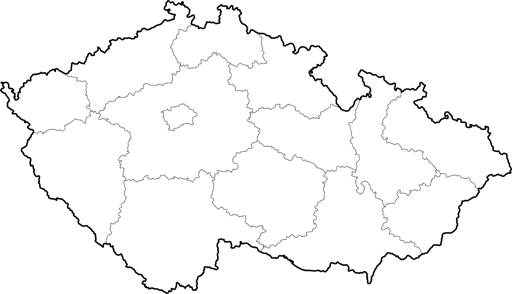
\includegraphics[width=0.5\textwidth]{files/map-coloring-czechia.png} \vfill
        
        \item A harder instance  
        
        \vfill 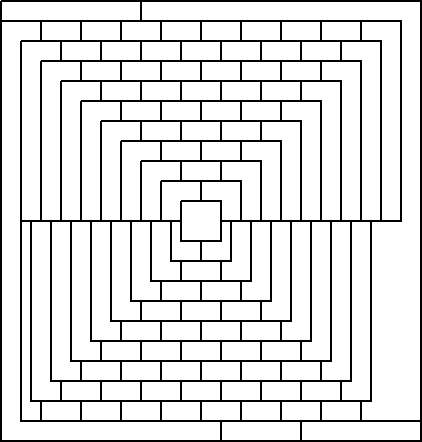
\includegraphics[width=0.33\textwidth]{files/map-coloring-hard.png} \vfill
    \end{enumerate}
    \end{multicols}

\end{problem}



\section*{For further thought}
    
    
\begin{problem} 
    
    For a given formula $\varphi$ in CNF, find a 3-CNF formula $\varphi'$ such that $\varphi'$ is satisfiable if and only if $\varphi$ is satisfiable. Describe an efficient algorithm for constructing $\varphi'$ given $\varphi$ (i.e., a \emph{reduction} from the SAT problem to the 3-SAT problem).

\end{problem}


\begin{problem}
    Encode the problem of sorting a given $n$-tuple of integers into SAT.
\end{problem}

\begin{problem}
    Encode into SAT the well-known riddle about a farmer who needs to transport a wolf, a goat, and a cabbage across a river.
\end{problem}

